
\section{Verschiedene Probleme}

\subsubsection{Ölbohrtürme}

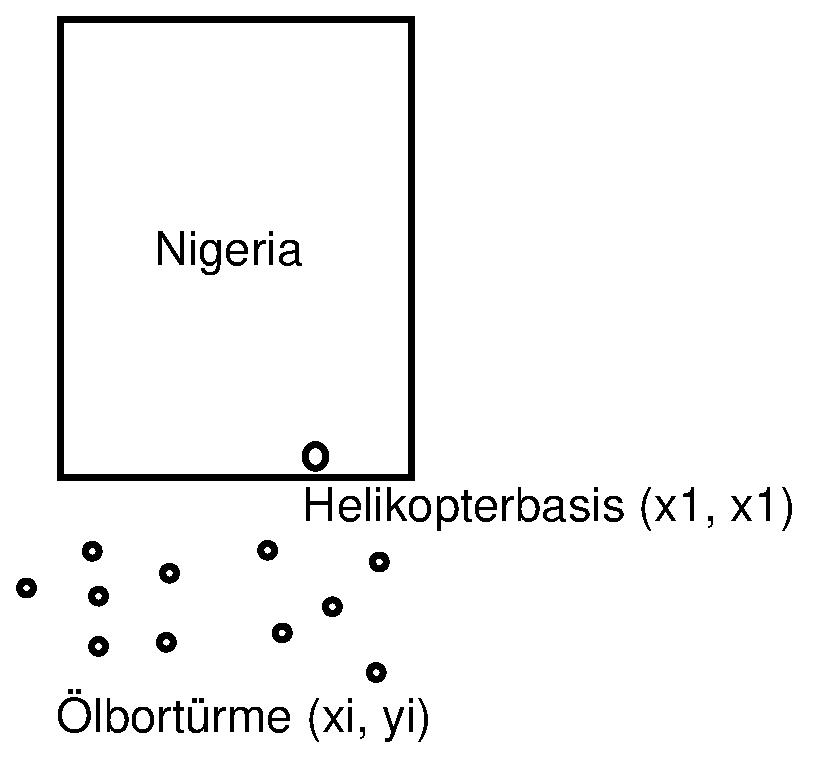
\includegraphics[width=5cm]{bilder/1-1Nigeria}

Der Helikopter fliegt eine vorgegebene Menge von Ölbohrtürmen ab um die
Pumpmenge zu regulieren und fliegt danach zurück zur Basis. Die Zeit, die
er dafür benötigt ist proportional zur Flugstrecke (euklidische Distanzen):
\[t(i,j) = \sqrt{(x_{i} - x_{j})^{2} + (y_{i} - y_{j})^{2}} = t(j,i)\]
Im Gegensatz dazu hat das Leiterplatten-Problem die $L_{\infty}$-Metrik die
auch Max Metrik genannt wird weil immer die maximale Strecke der beiden
strecken in x oder y Richtung genommen wird. Der Bohrer wird von zwei
Motoren über die Platine gefahren, die unabhängig voneinander ein und
ausgeschaltet werden können.

\subsubsection{Euklidisches Rundreise-Problem}

{\bf Gegeben:} Menge $V$ von Punkten in der euklidischen Ebene.\\
{\bf Gesucht:} Eine Tour minimaler Länge
\[n = |V| \hspace{10mm} \frac{(n-1)!}{2} \mbox{ mögliche Touren}\]

Für den Fall dass $n=23$ bräuchte ein Computer für die Auswertung einer
Tour $1\eta$s ($=10^{-9}$s) $\rightarrow$ Computer braucht zirka 178
Jahrhunderte zur Bewertung aller Touren.

\subsubsection{Plotten zusammenhängender Zeichnungen}

Das plotten eines Straßennetzes auf einer 60x60 cm Platte\\
Länge des Straßennetzes: 44,47m\\
Die Standard-Plottersoftware legte 67 km zurück und brauchte 9 Stunden und
11 Minuten.

Alternativ wurden die zu plottenden Strecken von einer "`intelligenten"'
Person durchgeführt.\\
Leerstrecke: 57,8 m\\
Zeit: 51 min

Nach Anwendung einer Matching Heuristik:
Leerstrecke: 13,62 m\\
Zeit: 36 min 45 sek.

\paragraph{Kleine Übungsaufgabe} In jedem Graphen ist die Anzahl der Punkte
mit ungerader Anzahl ein- und ausgehender Kanten gerade (Ein Satz von Euler). 

Nach Euler gilt auch, dass man einen Graphen genau dann ohne abzusetzen
und ohne eine Strecke zwei mal zu gehen zeichnen kann wenn die Anzahl der
Kanten an jedem Knoten gerade ist (einmal muss man rein, einmal raus,
falls man noch einmal rein geht, muss man auch wieder raus).

Das hilft uns nun beim Plot-Problem wir suchen nun die minimale Paarung
"`ungerader"' Knoten (die Gesamtlänge der verbindenden Kanten soll minimal
sein).

\subsubsection{Andere Rundreise-Probleme}

\paragraph{Chinesisches Postboten-Problem:} Dasselbe Problem wie beim
Plotten aber auf dünnen Graphen (Graphen mit relativ wenig Kanten).

\paragraph{Landpostboten-Problem:} Der Landpostboten muss sowohl in den
Dörfern möglichst optimal laufen als auch die Dörfer möglichst Optimal
abfahren. Das Euklidische Rundreise Problem ist hiervon ein Spezialfall
(wenn pro Dorf nur ein Haus beliefert werden muss).

\subsubsection{Euklidisches perfektes Matching-Problem}

{\bf Gegeben:} Menge $V$ von Punkten in der Euklidischen Ebene $|V|$ gerade.\\
{\bf Gesucht:} Eine Menge von Geraden Linien minimaler Gesamtlänge so dass
jeder Punkt Endpunkt genau einer Linie ist.

\section{Dualität und Schranken}

TSP-Versuch (Travelling Salesman oder eukl. Rundreise-Problem).

[Zeichnung]

Die Zeichnung stellt eine Menge von Punkten die durch Kanten verbunden sind
so dass eine Rundreise entsteht um alle Punkte herum sind nun Kreise, die
sich nicht überschneiden sondern sich falls ihre Mittelpunkte Nachbarn auf der Rundreise sind  lediglich berühren, bis auf eine
Stelle, wo eine Lücke entsteht. Jeder Kreis wird nun  genau 2 mal
durchlaufen + das eine Stück wo eine Lücke ist. Damit ist die Summe aller
Kreisdurchmesser + das extra Stück eine untere Schranke. Falls man es
schafft die Kreise so anzuordnen, dass sie sich nicht überschneiden aber
Nachbarn sich immer berühren so hat man die Optimallösung.

Oft ist aber auch keine Kombination der Kreise möglich.

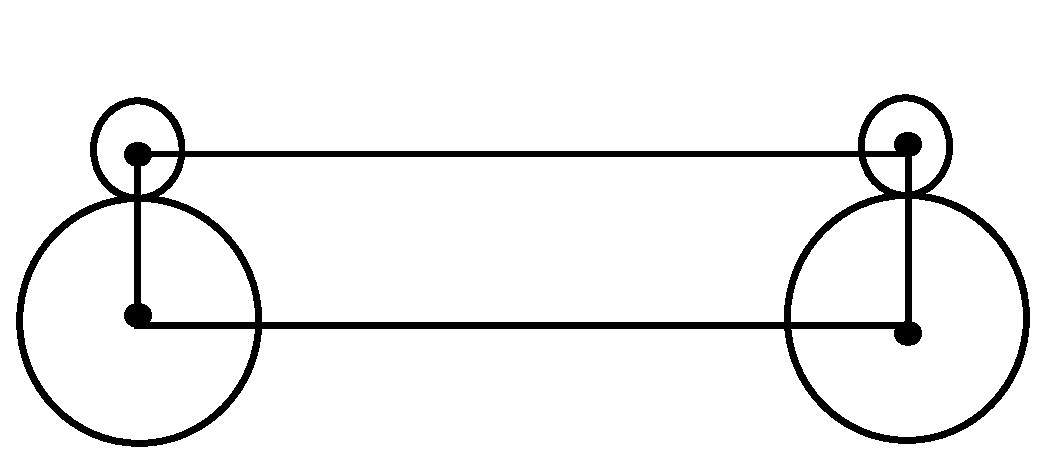
\includegraphics[width=8cm]{bilder/1-2Kreisegehtnicht}

In diesem Fall kann man dann Punkte zusammenfassen und mit "`Gräben"'


[3 Zeichnungen] habe ich leider nur ansatzweise und nicht die Zeit sie am
Computer nach zu zeichnen.

An das Euklidische Matching-Problem kann man ebenfalls mit dieser Methode
heran gehen.

\subsubsection{Euklidisches Rundreise untere Schranken Problem}

{\bf Gegeben:} Menge $V$ von Punkten in der euklidischen Ebene.\\
{\bf Gesucht:} nicht überlappendes System von Scheiben und Gräben das:
\[B=2 \sum_{v\in V} r_{v} + 2 \sum_{m\in M} w_{m}\]
maximiert.

\subsubsection{Euklidisches perf. Matching untere Schranken Problem}

{\bf Gegeben:} Menge $V$ von Punkten in der euklidischen Ebene. $|V|$
gerade.\\
{\bf Gesucht:} nicht überlappendes System von Scheiben und Gräben das:
\[\bar{B}= \sum_{v\in V} r_{v} + \sum_{m\in M} w_{m}\]
maximiert.
 
In der $L_{\infty}$-Matrix nimmt man Quadrate.

\subsection{Lineare Optimierung und untere Schranke Probleme}

\subsubsection{Euklidisches Rundreise-Problem nur mit Scheiben}

Als LP formuliert sieht es so aus:

\[\begin{array}{rcl}
(P_{1}) \hspace{7mm}  \max \displaystyle \sum_{u \in V} 2r_{u}\\
r_{u} + r_{v} &\leqq& t(u,\; v) \mbox{, für alle Paare }\{u,\; v\}\\
r_{u} &\geqq&0 \; \; \; \forall n\in V
\end{array}
\]

Das Duale LP lautet folgendermaßen:

\[\begin{array}{rcl}
(D_{1}) \hspace{7mm} \min \displaystyle \sum_{u,v} t(u,v) x_{u v}\\
\displaystyle \sum_{v\not= u} x_{u v} &\geqq & 2 \; \; \forall u \in V\\
x_{u v} &\geqq & 0 \mbox{, für alle Paare } \{u,\; v\} 
\end{array}\]

Beispiel mit vier Städten:\\\nopagebreak
\[\begin{array}{rcl}
\max \mat{rrrr}{2&2&2&2} \vect{r_{1}\\r_{2}\\r_{3}\\r_{4}}\\
s.t. \hspace {4mm} \mat{rrrr}{1&1&&\\1&&1&\\1&&&1\\&1&1&\\&1&&1\\&&1&1}
\vect{r_{1}\\r_{2}\\r_{3}\\r_{4}}
&\leqq&\vect{t(1,2)\\t(1,3)\\t(1,4)\\t(2,3)\\t(2,4)\\t(3,4)}\\
\vect{r_{1}\\r_{2}\\r_{3}\\r_{4}} &\geqq& 0
\end{array}\]

Dual

\[\begin{array}{rcl}
\min \; t(1,2)+\ldots+t(3,4) \vect{x_{12}\\\vdots\\x_{34}}\\
\mat{rrr}{x_{12}&\ldots&x_{34}}
\mat{rrrr}{1&1&&\\1&&1&\\1&&&1\\&1&1&\\&1&&1\\&&1&1} &\geqq&
\vect{2\\2\\2\\2}\\
x&\geqq& 0
\end{array}\]

\subsubsection{Hinzufügen von Gräben}

\[\begin{array}{rcl}
(P_{2}) \hspace{7mm}  \max \displaystyle \sum_{u \in V} 2r_{u}
+ \sum_{s\in M} 2 w_{s}\\
r_{u} + r_{v} + \displaystyle \sum_{s \in M, \; \left| \{u,v\} \cap s 
\right| =1} w_{s}&\leqq& t(u,\; v) \mbox{, für alle Paare }\{u,\; v\}\\
r_{u} &\geqq&0 \; \; \; \forall u\in V\\
w_{s} &\geqq& 0 \; \; \; \forall s \in M
\end{array}
\]

Das Duale LP lautet folgendermaßen:

\[\begin{array}{rcl}
(D_{2}) \hspace{7mm} \min \displaystyle \sum_{u,v} t(u,v) x_{u v}\\
\displaystyle \sum_{v\not= u} x_{u v} &\geqq & 2 \; \; \forall u \in V\\
\displaystyle \sum_{\left| \{u,v\} \cap s \right| =1} x_{u v} &\geqq& 2  \;
\; \forall s \in M\\
x_{u v} &\geqq & 0 \mbox{, für alle Paare } \{u,\; v\} 
\end{array}\]

Für jede Tour T erfüllt der Inzidenzvektor $\bar{X}$ die Restriktionen von 
$(D_{2})$.\\
$\stackrel{\mbox{\scriptsize Schwache Dualität}}{\Rightarrow}$ Die Optimallösung
für $(D_{2})$ ist eine untere Schranke für die Länge einer Tour. Wenn man
mehr Ungleichungen zu $(D_{2})$ hinzufügt erhält man eine bessere untere
Schranke ($\rightarrow$ nächstes Semester).

\paragraph{Analoge Konstruktion} für perfektes euklidisches Matching

$O$ ist die Familie der Teilmengen von $V$ ungerader Kardinalität.
\[\begin{array}{rcl}
(P_{2}) \hspace{7mm}  \max \displaystyle \sum_{u \in V} r_{u}
+ \sum_{s\in O}  w_{s}\\
r_{u} + r_{v} + \displaystyle \sum_{s \in O, \; \left| \{u,v\} \cap s
\right| =1} w_{s}&\leqq& t(u,\; v) \mbox{, für alle Paare }\{u,\; v\}\\
r_{u} &\geqq&0 \; \; \; \forall u\in V\\
w_{s} &\geqq& 0 \; \; \; \forall s \in O
\end{array}
\]

Das Duale LP lautet folgendermaßen:

\[\begin{array}{rcl}
(D_{2}) \hspace{7mm} \min \displaystyle \sum_{u,v} t(u,v) x_{u v}\\
\displaystyle \sum_{v\not= u} x_{u v} &\geqq & 1 \; \; \forall u \in V\\
\displaystyle \sum_{\left| \{u,v\} \cap s \right| =1} x_{u v} &\geqq& 1 \;
\; \forall s \in O\\
x_{u v} &\geqq & 0 \mbox{, für alle Paare } \{u,\; v\} 
\end{array}\]

Für alle $x_{u v}$ > 0 sind die entsprechenden dualen Ungleichungen mit
Gleichheit erfüllt.
Optimalität durch schwache Dualität und komplementären Schlupf.


